% Options for packages loaded elsewhere
\PassOptionsToPackage{unicode}{hyperref}
\PassOptionsToPackage{hyphens}{url}
\PassOptionsToPackage{dvipsnames,svgnames,x11names}{xcolor}
%
\documentclass[
  letterpaper,
  DIV=11,
  numbers=noendperiod]{scrreprt}

\usepackage{amsmath,amssymb}
\usepackage{iftex}
\ifPDFTeX
  \usepackage[T1]{fontenc}
  \usepackage[utf8]{inputenc}
  \usepackage{textcomp} % provide euro and other symbols
\else % if luatex or xetex
  \usepackage{unicode-math}
  \defaultfontfeatures{Scale=MatchLowercase}
  \defaultfontfeatures[\rmfamily]{Ligatures=TeX,Scale=1}
\fi
\usepackage{lmodern}
\ifPDFTeX\else  
    % xetex/luatex font selection
\fi
% Use upquote if available, for straight quotes in verbatim environments
\IfFileExists{upquote.sty}{\usepackage{upquote}}{}
\IfFileExists{microtype.sty}{% use microtype if available
  \usepackage[]{microtype}
  \UseMicrotypeSet[protrusion]{basicmath} % disable protrusion for tt fonts
}{}
\makeatletter
\@ifundefined{KOMAClassName}{% if non-KOMA class
  \IfFileExists{parskip.sty}{%
    \usepackage{parskip}
  }{% else
    \setlength{\parindent}{0pt}
    \setlength{\parskip}{6pt plus 2pt minus 1pt}}
}{% if KOMA class
  \KOMAoptions{parskip=half}}
\makeatother
\usepackage{xcolor}
\setlength{\emergencystretch}{3em} % prevent overfull lines
\setcounter{secnumdepth}{5}
% Make \paragraph and \subparagraph free-standing
\makeatletter
\ifx\paragraph\undefined\else
  \let\oldparagraph\paragraph
  \renewcommand{\paragraph}{
    \@ifstar
      \xxxParagraphStar
      \xxxParagraphNoStar
  }
  \newcommand{\xxxParagraphStar}[1]{\oldparagraph*{#1}\mbox{}}
  \newcommand{\xxxParagraphNoStar}[1]{\oldparagraph{#1}\mbox{}}
\fi
\ifx\subparagraph\undefined\else
  \let\oldsubparagraph\subparagraph
  \renewcommand{\subparagraph}{
    \@ifstar
      \xxxSubParagraphStar
      \xxxSubParagraphNoStar
  }
  \newcommand{\xxxSubParagraphStar}[1]{\oldsubparagraph*{#1}\mbox{}}
  \newcommand{\xxxSubParagraphNoStar}[1]{\oldsubparagraph{#1}\mbox{}}
\fi
\makeatother

\usepackage{color}
\usepackage{fancyvrb}
\newcommand{\VerbBar}{|}
\newcommand{\VERB}{\Verb[commandchars=\\\{\}]}
\DefineVerbatimEnvironment{Highlighting}{Verbatim}{commandchars=\\\{\}}
% Add ',fontsize=\small' for more characters per line
\usepackage{framed}
\definecolor{shadecolor}{RGB}{241,243,245}
\newenvironment{Shaded}{\begin{snugshade}}{\end{snugshade}}
\newcommand{\AlertTok}[1]{\textcolor[rgb]{0.68,0.00,0.00}{#1}}
\newcommand{\AnnotationTok}[1]{\textcolor[rgb]{0.37,0.37,0.37}{#1}}
\newcommand{\AttributeTok}[1]{\textcolor[rgb]{0.40,0.45,0.13}{#1}}
\newcommand{\BaseNTok}[1]{\textcolor[rgb]{0.68,0.00,0.00}{#1}}
\newcommand{\BuiltInTok}[1]{\textcolor[rgb]{0.00,0.23,0.31}{#1}}
\newcommand{\CharTok}[1]{\textcolor[rgb]{0.13,0.47,0.30}{#1}}
\newcommand{\CommentTok}[1]{\textcolor[rgb]{0.37,0.37,0.37}{#1}}
\newcommand{\CommentVarTok}[1]{\textcolor[rgb]{0.37,0.37,0.37}{\textit{#1}}}
\newcommand{\ConstantTok}[1]{\textcolor[rgb]{0.56,0.35,0.01}{#1}}
\newcommand{\ControlFlowTok}[1]{\textcolor[rgb]{0.00,0.23,0.31}{\textbf{#1}}}
\newcommand{\DataTypeTok}[1]{\textcolor[rgb]{0.68,0.00,0.00}{#1}}
\newcommand{\DecValTok}[1]{\textcolor[rgb]{0.68,0.00,0.00}{#1}}
\newcommand{\DocumentationTok}[1]{\textcolor[rgb]{0.37,0.37,0.37}{\textit{#1}}}
\newcommand{\ErrorTok}[1]{\textcolor[rgb]{0.68,0.00,0.00}{#1}}
\newcommand{\ExtensionTok}[1]{\textcolor[rgb]{0.00,0.23,0.31}{#1}}
\newcommand{\FloatTok}[1]{\textcolor[rgb]{0.68,0.00,0.00}{#1}}
\newcommand{\FunctionTok}[1]{\textcolor[rgb]{0.28,0.35,0.67}{#1}}
\newcommand{\ImportTok}[1]{\textcolor[rgb]{0.00,0.46,0.62}{#1}}
\newcommand{\InformationTok}[1]{\textcolor[rgb]{0.37,0.37,0.37}{#1}}
\newcommand{\KeywordTok}[1]{\textcolor[rgb]{0.00,0.23,0.31}{\textbf{#1}}}
\newcommand{\NormalTok}[1]{\textcolor[rgb]{0.00,0.23,0.31}{#1}}
\newcommand{\OperatorTok}[1]{\textcolor[rgb]{0.37,0.37,0.37}{#1}}
\newcommand{\OtherTok}[1]{\textcolor[rgb]{0.00,0.23,0.31}{#1}}
\newcommand{\PreprocessorTok}[1]{\textcolor[rgb]{0.68,0.00,0.00}{#1}}
\newcommand{\RegionMarkerTok}[1]{\textcolor[rgb]{0.00,0.23,0.31}{#1}}
\newcommand{\SpecialCharTok}[1]{\textcolor[rgb]{0.37,0.37,0.37}{#1}}
\newcommand{\SpecialStringTok}[1]{\textcolor[rgb]{0.13,0.47,0.30}{#1}}
\newcommand{\StringTok}[1]{\textcolor[rgb]{0.13,0.47,0.30}{#1}}
\newcommand{\VariableTok}[1]{\textcolor[rgb]{0.07,0.07,0.07}{#1}}
\newcommand{\VerbatimStringTok}[1]{\textcolor[rgb]{0.13,0.47,0.30}{#1}}
\newcommand{\WarningTok}[1]{\textcolor[rgb]{0.37,0.37,0.37}{\textit{#1}}}

\providecommand{\tightlist}{%
  \setlength{\itemsep}{0pt}\setlength{\parskip}{0pt}}\usepackage{longtable,booktabs,array}
\usepackage{calc} % for calculating minipage widths
% Correct order of tables after \paragraph or \subparagraph
\usepackage{etoolbox}
\makeatletter
\patchcmd\longtable{\par}{\if@noskipsec\mbox{}\fi\par}{}{}
\makeatother
% Allow footnotes in longtable head/foot
\IfFileExists{footnotehyper.sty}{\usepackage{footnotehyper}}{\usepackage{footnote}}
\makesavenoteenv{longtable}
\usepackage{graphicx}
\makeatletter
\newsavebox\pandoc@box
\newcommand*\pandocbounded[1]{% scales image to fit in text height/width
  \sbox\pandoc@box{#1}%
  \Gscale@div\@tempa{\textheight}{\dimexpr\ht\pandoc@box+\dp\pandoc@box\relax}%
  \Gscale@div\@tempb{\linewidth}{\wd\pandoc@box}%
  \ifdim\@tempb\p@<\@tempa\p@\let\@tempa\@tempb\fi% select the smaller of both
  \ifdim\@tempa\p@<\p@\scalebox{\@tempa}{\usebox\pandoc@box}%
  \else\usebox{\pandoc@box}%
  \fi%
}
% Set default figure placement to htbp
\def\fps@figure{htbp}
\makeatother
% definitions for citeproc citations
\NewDocumentCommand\citeproctext{}{}
\NewDocumentCommand\citeproc{mm}{%
  \begingroup\def\citeproctext{#2}\cite{#1}\endgroup}
\makeatletter
 % allow citations to break across lines
 \let\@cite@ofmt\@firstofone
 % avoid brackets around text for \cite:
 \def\@biblabel#1{}
 \def\@cite#1#2{{#1\if@tempswa , #2\fi}}
\makeatother
\newlength{\cslhangindent}
\setlength{\cslhangindent}{1.5em}
\newlength{\csllabelwidth}
\setlength{\csllabelwidth}{3em}
\newenvironment{CSLReferences}[2] % #1 hanging-indent, #2 entry-spacing
 {\begin{list}{}{%
  \setlength{\itemindent}{0pt}
  \setlength{\leftmargin}{0pt}
  \setlength{\parsep}{0pt}
  % turn on hanging indent if param 1 is 1
  \ifodd #1
   \setlength{\leftmargin}{\cslhangindent}
   \setlength{\itemindent}{-1\cslhangindent}
  \fi
  % set entry spacing
  \setlength{\itemsep}{#2\baselineskip}}}
 {\end{list}}
\usepackage{calc}
\newcommand{\CSLBlock}[1]{\hfill\break\parbox[t]{\linewidth}{\strut\ignorespaces#1\strut}}
\newcommand{\CSLLeftMargin}[1]{\parbox[t]{\csllabelwidth}{\strut#1\strut}}
\newcommand{\CSLRightInline}[1]{\parbox[t]{\linewidth - \csllabelwidth}{\strut#1\strut}}
\newcommand{\CSLIndent}[1]{\hspace{\cslhangindent}#1}

\KOMAoption{captions}{tableheading}
\makeatletter
\@ifpackageloaded{bookmark}{}{\usepackage{bookmark}}
\makeatother
\makeatletter
\@ifpackageloaded{caption}{}{\usepackage{caption}}
\AtBeginDocument{%
\ifdefined\contentsname
  \renewcommand*\contentsname{Table of contents}
\else
  \newcommand\contentsname{Table of contents}
\fi
\ifdefined\listfigurename
  \renewcommand*\listfigurename{List of Figures}
\else
  \newcommand\listfigurename{List of Figures}
\fi
\ifdefined\listtablename
  \renewcommand*\listtablename{List of Tables}
\else
  \newcommand\listtablename{List of Tables}
\fi
\ifdefined\figurename
  \renewcommand*\figurename{Figure}
\else
  \newcommand\figurename{Figure}
\fi
\ifdefined\tablename
  \renewcommand*\tablename{Table}
\else
  \newcommand\tablename{Table}
\fi
}
\@ifpackageloaded{float}{}{\usepackage{float}}
\floatstyle{ruled}
\@ifundefined{c@chapter}{\newfloat{codelisting}{h}{lop}}{\newfloat{codelisting}{h}{lop}[chapter]}
\floatname{codelisting}{Listing}
\newcommand*\listoflistings{\listof{codelisting}{List of Listings}}
\makeatother
\makeatletter
\makeatother
\makeatletter
\@ifpackageloaded{caption}{}{\usepackage{caption}}
\@ifpackageloaded{subcaption}{}{\usepackage{subcaption}}
\makeatother

\usepackage{bookmark}

\IfFileExists{xurl.sty}{\usepackage{xurl}}{} % add URL line breaks if available
\urlstyle{same} % disable monospaced font for URLs
\hypersetup{
  pdftitle={Data Mining},
  pdfauthor={Thiyanga S. Talagala},
  colorlinks=true,
  linkcolor={blue},
  filecolor={Maroon},
  citecolor={Blue},
  urlcolor={Blue},
  pdfcreator={LaTeX via pandoc}}


\title{Data Mining}
\author{Thiyanga S. Talagala}
\date{2025-10-11}

\begin{document}
\maketitle

\renewcommand*\contentsname{Table of contents}
{
\hypersetup{linkcolor=}
\setcounter{tocdepth}{2}
\tableofcontents
}

\bookmarksetup{startatroot}

\chapter*{Preface}\label{preface}
\addcontentsline{toc}{chapter}{Preface}

\markboth{Preface}{Preface}

\bookmarksetup{startatroot}

\chapter{Introduction to Data Mining}\label{introduction-to-data-mining}

\section{What is Data Mining?}\label{what-is-data-mining}

• Process of discovering interesting patterns of knowledge from huge
amounts of data.

\section{What do we mean by interesting
patterns?}\label{what-do-we-mean-by-interesting-patterns}

• Interesting patterns: Valid, Novel, Useful, Understandable

Example

• Retailers collect data about customer purchases at the checkout
counters

• Customer purchasing patterns: Identify which items are frequently sold
together?

• Products that are likely to be purchased together.

Why it is useful?

• Can make a purchase suggestion to their customers

• Gives an idea that how we can arrange items in a store to as a
strategy for boosting sales.

\section{Characteristics of Big Data: 5 V's of Big
Data}\label{characteristics-of-big-data-5-vs-of-big-data}

\begin{enumerate}
\def\labelenumi{\arabic{enumi}.}
\item
  Volume: size
\item
  Velocity: how quickly data is generated?
\item
  Variety: diversity
\item
  Veracity: quality of data
\item
  Value: how useful?
\end{enumerate}

\section{What motivates the development of data mining
field?}\label{what-motivates-the-development-of-data-mining-field}

• Scalability

• High dimensionality

• Heterogeneous and complex data

• Data ownership and distribution

\section{Data Mining Tasks}\label{data-mining-tasks}

\begin{enumerate}
\def\labelenumi{\arabic{enumi}.}
\item
  Predictive tasks: Predict the value of a particular attribute based on
  the values of other attributes
\item
  Descriptive tasks: Find human-interpretable patterns that describe
  data
\end{enumerate}

\section{Data Quality}\label{data-quality}

\begin{enumerate}
\def\labelenumi{\arabic{enumi}.}
\item
  Range: How narrow or wide of the scope of these data?
\item
  Relevancy: Is the data relevant to the problem?
\item
  Recency: How recent the data is generated?
\item
  Robustness: Signal to noise ratio
\item
  Reliability: How accurate?
\end{enumerate}

\section{Applications}\label{applications}

\begin{enumerate}
\def\labelenumi{\arabic{enumi}.}
\item
  Web mining: recommendation systems
\item
  Screening images: Early warning of ecological disasters
\item
  Marketing and sales
\item
  Diagnosis
\item
  Load forecasting
\item
  Decision involving judgement
\end{enumerate}

Many more\ldots{}

\bookmarksetup{startatroot}

\chapter{What is Statistical
Learing?}\label{what-is-statistical-learing}

In-class explanations

\bookmarksetup{startatroot}

\chapter{Decision Trees}\label{decision-trees}

\section{Motivational Example
Dataset}\label{motivational-example-dataset}

Features: Sepal Length, Sepal Width

Outcome: Species: setosa/versicolor

\subsection{Predictor space}\label{predictor-space}

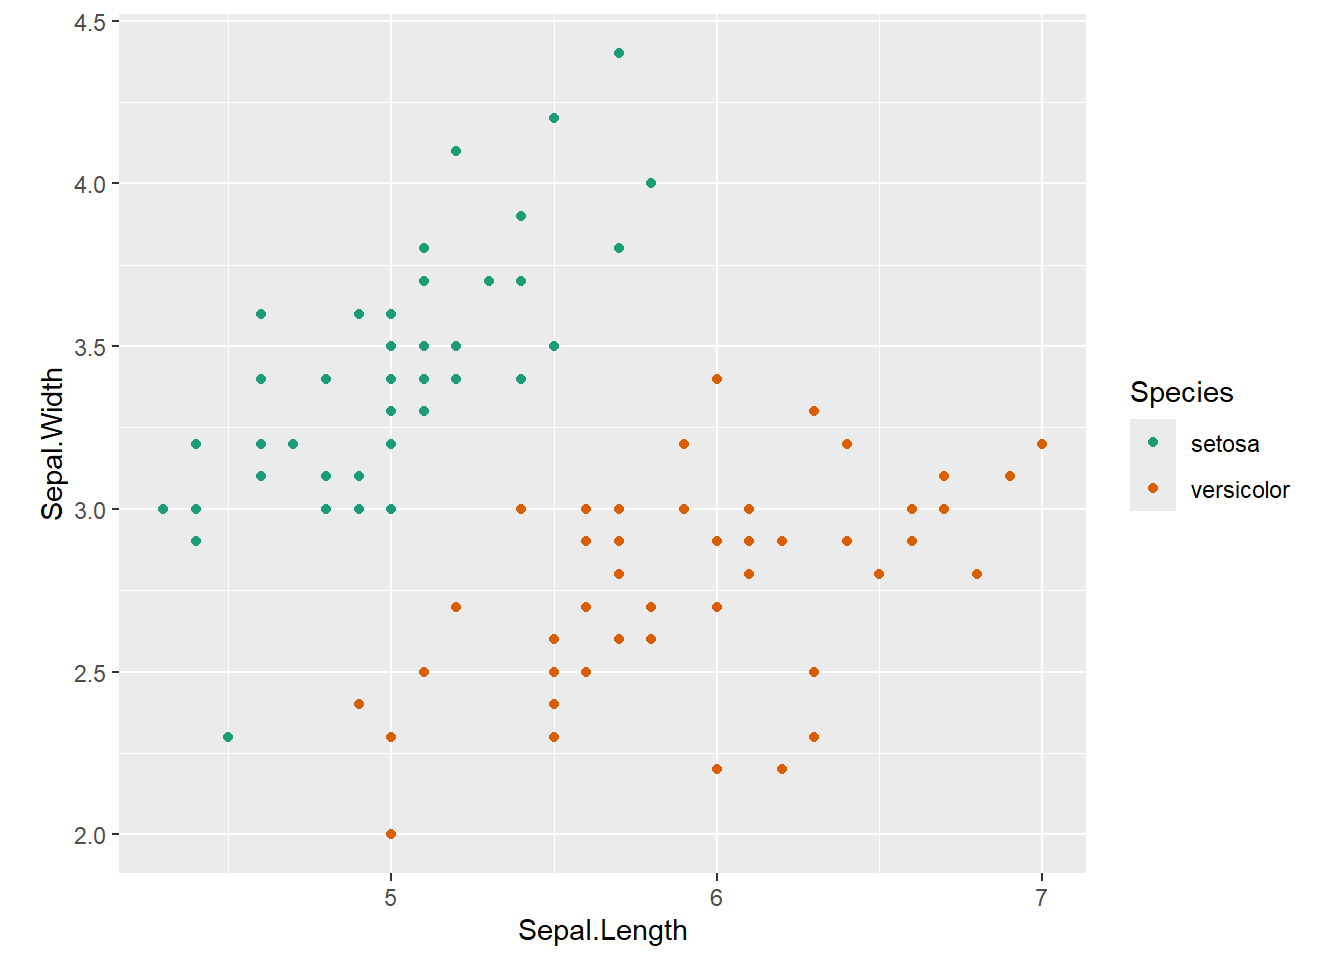
\includegraphics[width=\linewidth,height=0.7\textheight,keepaspectratio]{ch3_files/figure-pdf/unnamed-chunk-1-1.pdf}

\subsection{Decision Tree}\label{decision-tree}

\pandocbounded{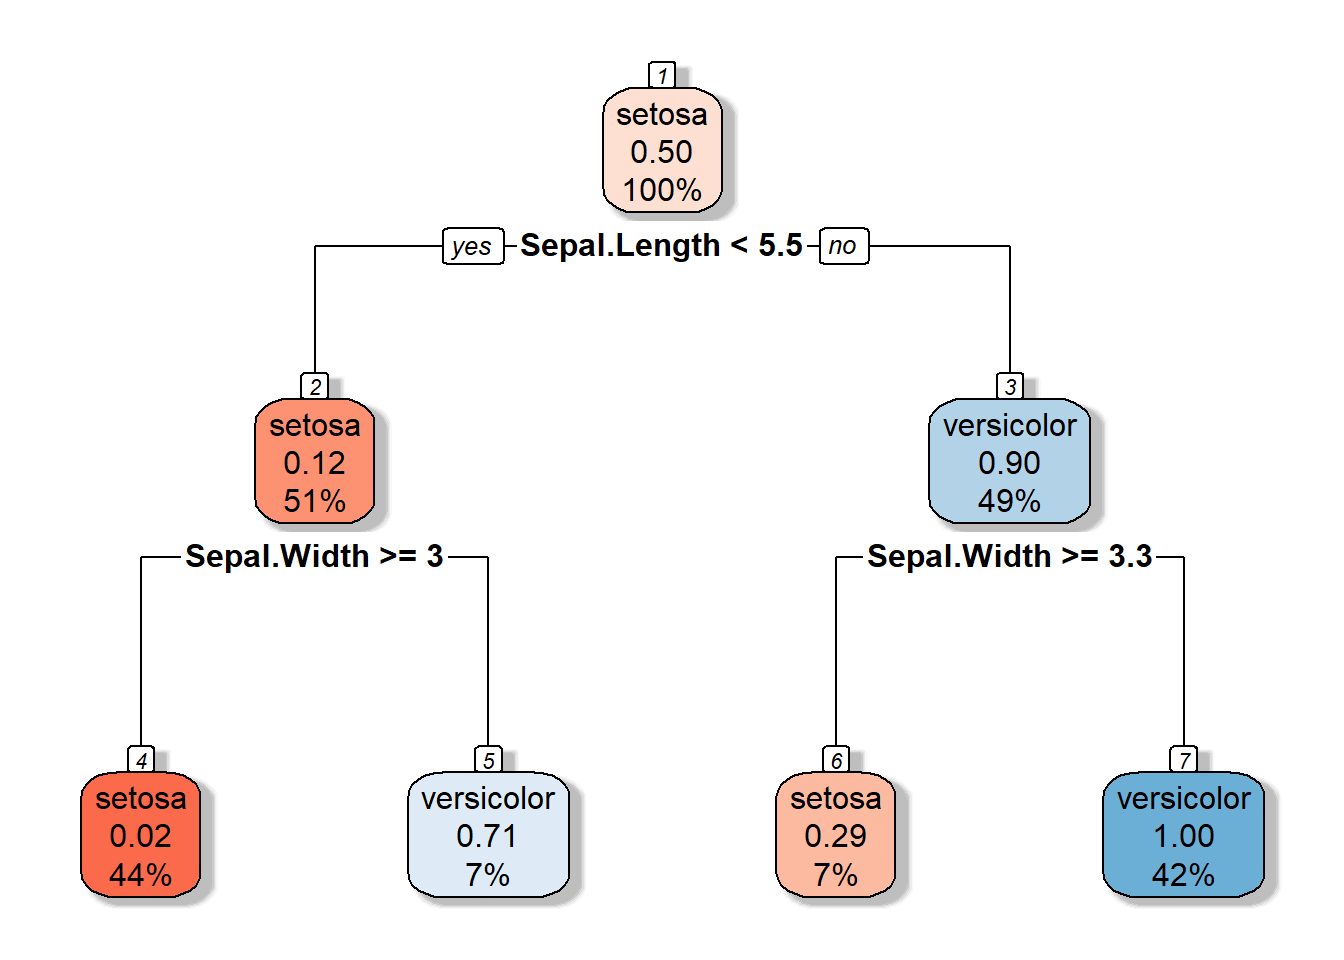
\includegraphics[keepaspectratio]{ch3_files/figure-pdf/unnamed-chunk-2-1.pdf}}

\subsection{Partition space}\label{partition-space}

\pandocbounded{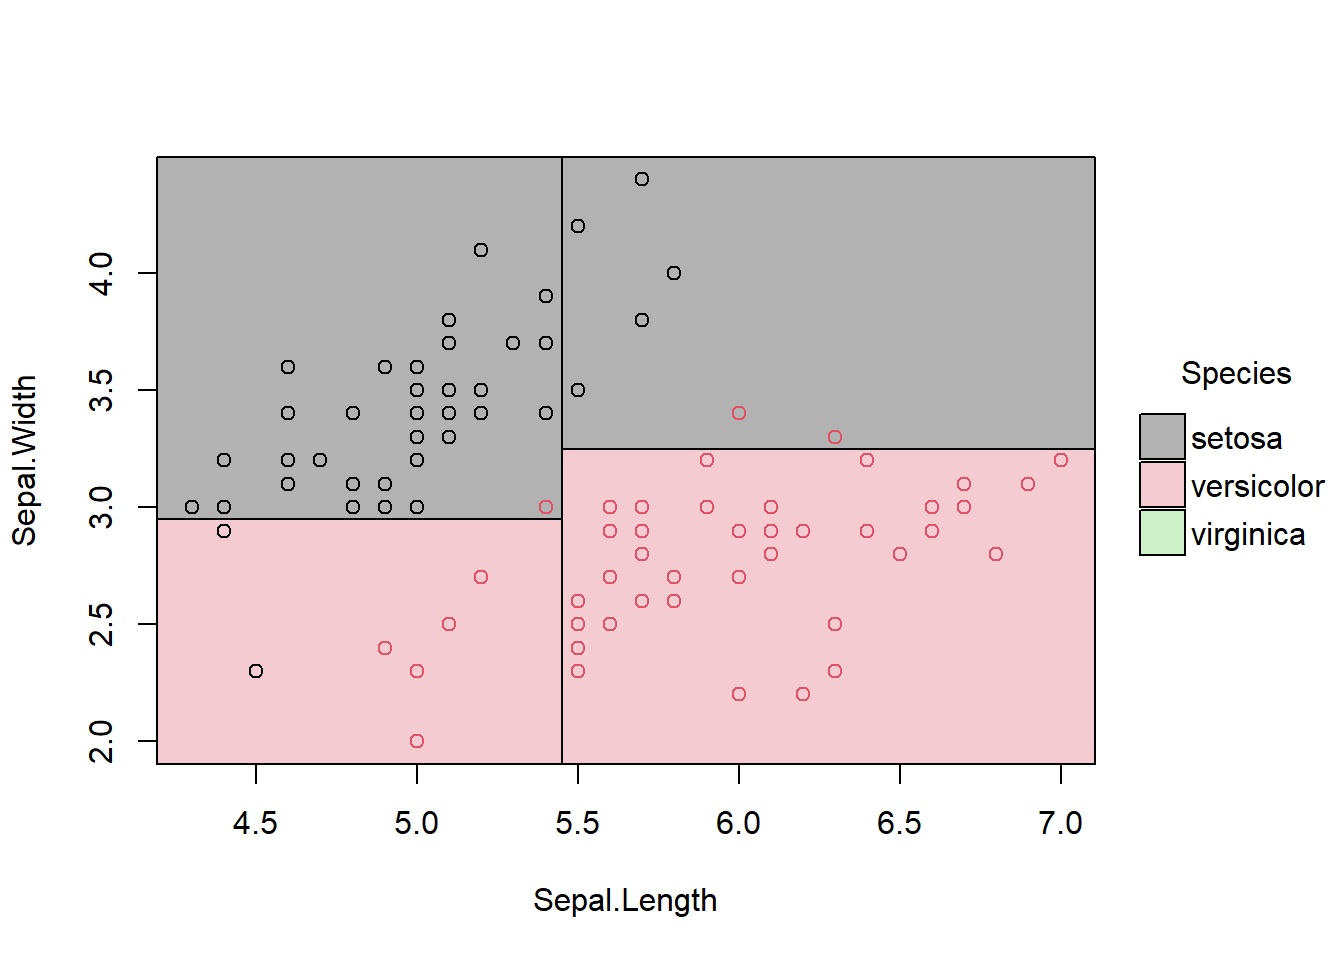
\includegraphics[keepaspectratio]{ch3_files/figure-pdf/unnamed-chunk-3-1.pdf}}

\pandocbounded{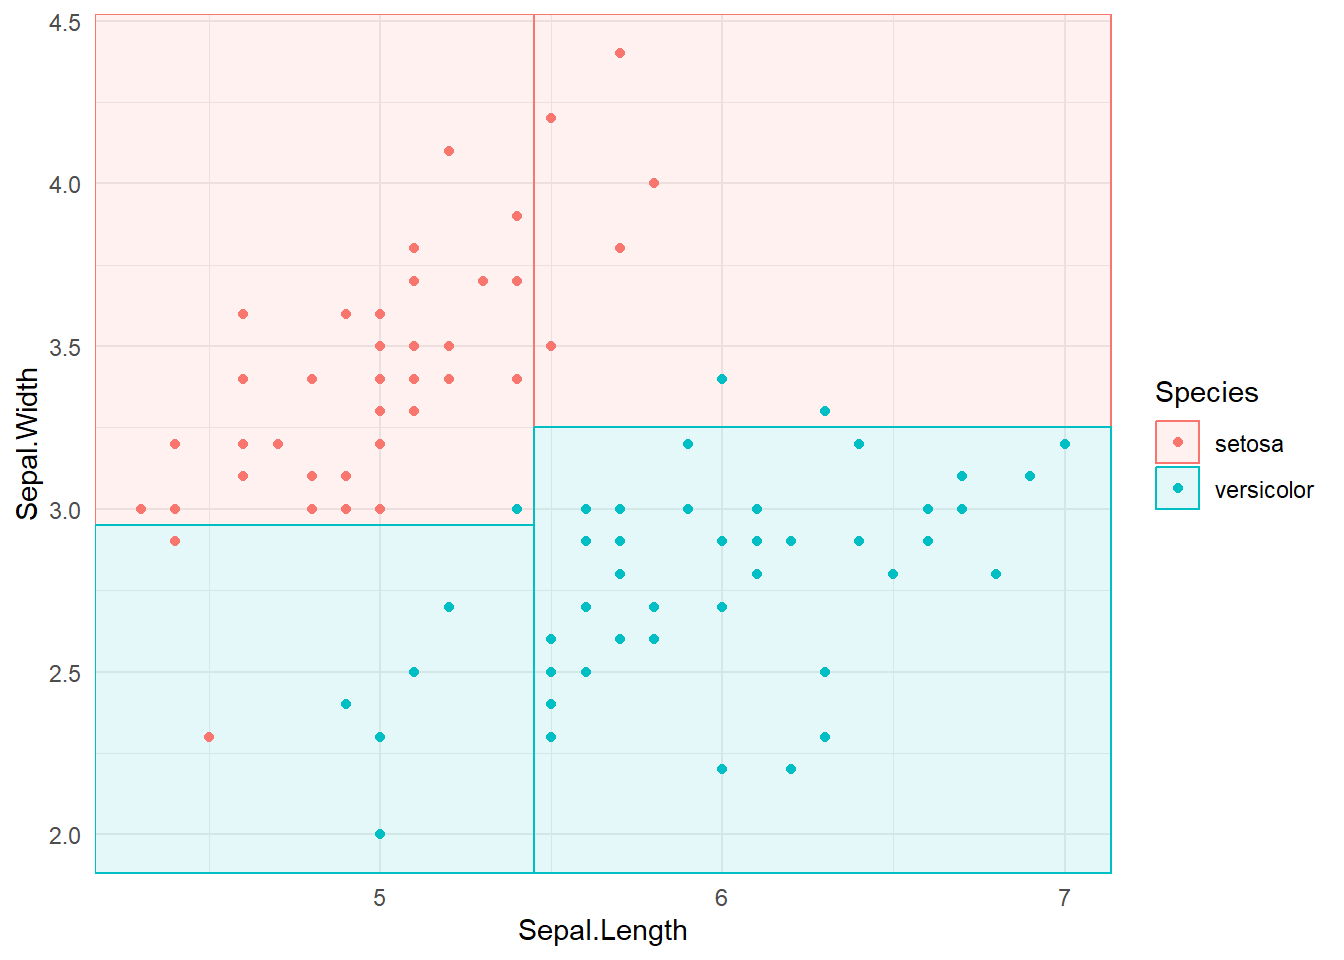
\includegraphics[keepaspectratio]{ch3_files/figure-pdf/unnamed-chunk-4-1.pdf}}

\(R1 = \{X|Sepal.Width >=3, Sepal.Length <5.5
\}\)

\section{Parts of a decision tree}\label{parts-of-a-decision-tree}

\begin{itemize}
\item
  Root node
\item
  Decision node
\item
  Terminal node/ Leaf node (gives outputs/class assignments)
\item
  Subtree
\end{itemize}

\section{Introduction}\label{introduction}

What happens in the model training phase?

\begin{itemize}
\item
  Stratify or segment the predictor space into a number of
  non-overlapping regions.
\item
  Set of splitting rules are used to segment the predictor space.
\item
  Decision tree consists of a series of splitting rules.
\end{itemize}

How to make predictions?

\begin{itemize}
\item
  Mean or mode response value for the training observations in the
  region which the observation we want to predict belong to.
\item
  We make the same prediction, for the training observations in the
  \(j^{th}\) region \(R_j\).
\end{itemize}

\section{Decision Trees: Regression - Finding the best split and best
splitting
variable}\label{decision-trees-regression---finding-the-best-split-and-best-splitting-variable}

The goal is to find \(R_1, R_2, R_3...R_J\), \(J\) distinct and
non-overlapping regions that minimize the RSS given by

\[\sum_{j=1}^{J}\sum_{i \in R_j}(y_i - \hat{y}_{R_j})^2.\]
\(\hat{y}_{R_j}\) - mean response for the training observations within
the \(j^{th}\) region.

In theory, to build the best possible decision tree, we could try every
possible way of splitting the data at every step and choose the one that
gives the best results. However, this is computationally infeasible,
especially when the dataset is large or when there are many predictor
variables --- the number of possible splits grows exponentially.

Therefore, instead of trying all possible combinations at once, we use a
\textbf{recursive partitioning approach}. This means:

Start with the entire dataset as one group (the root node).

Find the single best split --- the one that most effectively separates
the data based on the target variable.

Divide the data into two or more subgroups (child nodes) based on that
split.

Repeat the process (recursively) within each subgroup: again find the
best split, divide the data, and continue until a stopping rule is met
(for example, minimum node size or maximum tree depth).

This recursive process allows the algorithm to build the tree step by
step, finding locally optimal splits that approximate the best possible
tree without having to evaluate every possible combination.

\section{Recursive Partitioning for Regression
Trees}\label{recursive-partitioning-for-regression-trees}

A regression tree predicts a continuous outcome (for example, house
price, temperature, or pH level). The goal is to split the data into
smaller and smaller groups (nodes) that are as homogeneous as possible
with respect to the response variable.

In-class notation

\section{Recursive Partitioning for Regression
Trees}\label{recursive-partitioning-for-regression-trees-1}

A \textbf{regression tree} is used when the response variable is
\emph{continuous} (e.g., house price, temperature, or pH level).

The goal is to split the data into smaller and smaller groups (nodes)
that are as \textbf{homogeneous as possible} with respect to the
response.

\subsection{Step 1: Start with All
Predictors}\label{step-1-start-with-all-predictors}

At the beginning, the algorithm considers \textbf{all predictor
variables}:

\[X_1, X_2, X_3, \dots, X_p\]

For each predictor, it looks for the \textbf{best split point} that
divides the data into two groups such that the prediction error (usually
the \textbf{sum of squared errors, SSE}) is minimized.

\subsection{Step 2: Consider All Possible
Values}\label{step-2-consider-all-possible-values}

\subsubsection{Continuous predictors}\label{continuous-predictors}

If a predictor \(X_j\) is \textbf{continuous},\\
then ``all possible values'' refers to \textbf{all unique values} (or
\textbf{midpoints between consecutive sorted values}) that can be used
to split the data.

Example:

\begin{longtable}[]{@{}ll@{}}
\toprule\noalign{}
Observation & \(X_j\) \\
\midrule\noalign{}
\endhead
\bottomrule\noalign{}
\endlastfoot
1 & 2 \\
2 & 3 \\
3 & 5 \\
4 & 7 \\
\end{longtable}

Possible split points (midpoints): - \(X_j < 2.5\) - \(X_j < 4\) -
\(X_j < 6\)

Each of these potential splits is tested to see how well it reduces the
SSE of the response variable.

\subsubsection{Categorical predictors}\label{categorical-predictors}

If \(X_j\) is \textbf{categorical},\\
``all possible values'' means all possible \textbf{groupings (subsets)}
of the categories.

Example:\\
If the predictor \texttt{Species} = \{A, B, C\}, possible splits are:

\begin{itemize}
\item
  \{A\} vs \{B, C\}
\item
  \{B\} vs \{A, C\}
\item
  \{C\} vs \{A, B\}
\end{itemize}

Each grouping is evaluated based on how much it reduces the variability
in the response.

\subsection{Step 3: Choose the Best
Split}\label{step-3-choose-the-best-split}

For every predictor and every possible split value, compute:

\[
\text{SSE}_{\text{split}} = \text{SSE}_{\text{left node}} + \text{SSE}_{\text{right node}}
\]

The \textbf{split that minimizes} this total SSE is chosen as the best
split for that node.

\subsection{Step 4: Recursive
Partitioning}\label{step-4-recursive-partitioning}

After splitting the data into two nodes, the same process is applied
\textbf{recursively} within each node:

\begin{enumerate}
\def\labelenumi{\arabic{enumi}.}
\tightlist
\item
  Consider all predictors again.\\
\item
  For each predictor, test all possible values.\\
\item
  Find the best split within that node.\\
\item
  Continue until a stopping rule is met (e.g., minimum node size or no
  significant improvement).
\end{enumerate}

\subsection{Summary}\label{summary}

\begin{longtable}[]{@{}
  >{\raggedright\arraybackslash}p{(\linewidth - 2\tabcolsep) * \real{0.4167}}
  >{\raggedright\arraybackslash}p{(\linewidth - 2\tabcolsep) * \real{0.5833}}@{}}
\toprule\noalign{}
\begin{minipage}[b]{\linewidth}\raggedright
Concept
\end{minipage} & \begin{minipage}[b]{\linewidth}\raggedright
Explanation
\end{minipage} \\
\midrule\noalign{}
\endhead
\bottomrule\noalign{}
\endlastfoot
\textbf{All predictors} & Every variable \(X_1, X_2, \dots, X_p\) is
considered at each split. \\
\textbf{All possible values} & Every unique value (or midpoint between
values) is tested as a potential split. \\
\textbf{Recursive partitioning} & The process of repeatedly splitting
the data into smaller homogeneous groups until a stopping rule is
met. \\
\end{longtable}

\begin{quote}
\textbf{In summary:}\\
Finding every possible combination of splits is computationally
infeasible.\\
Recursive partitioning provides a practical, step-by-step method that
finds locally optimal splits efficiently.
\end{quote}

\section{Depth of the decision tree}\label{depth-of-the-decision-tree}

\pandocbounded{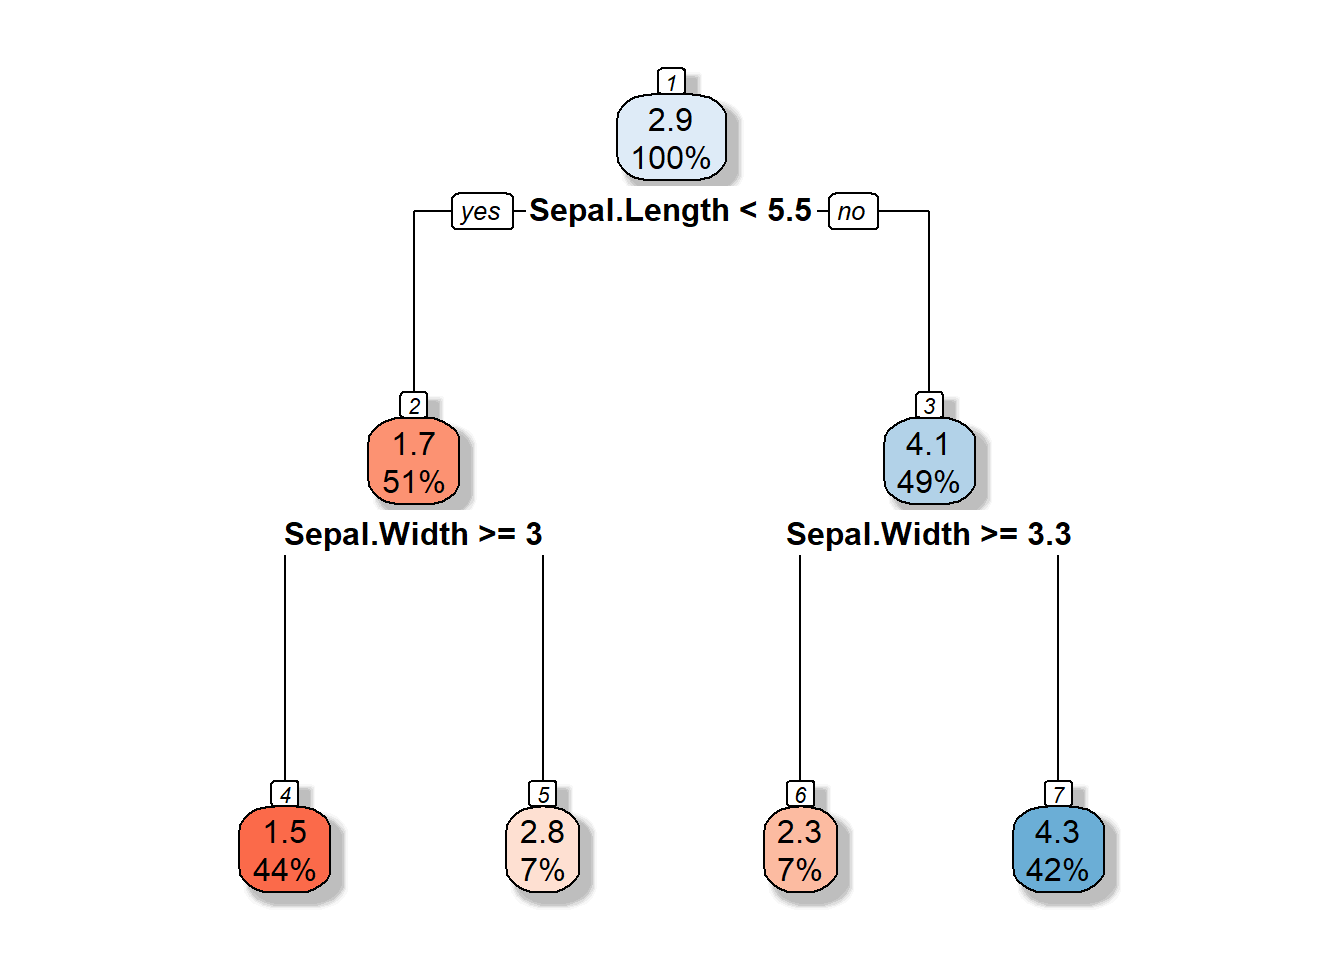
\includegraphics[keepaspectratio]{ch3_files/figure-pdf/unnamed-chunk-5-1.pdf}}

\pandocbounded{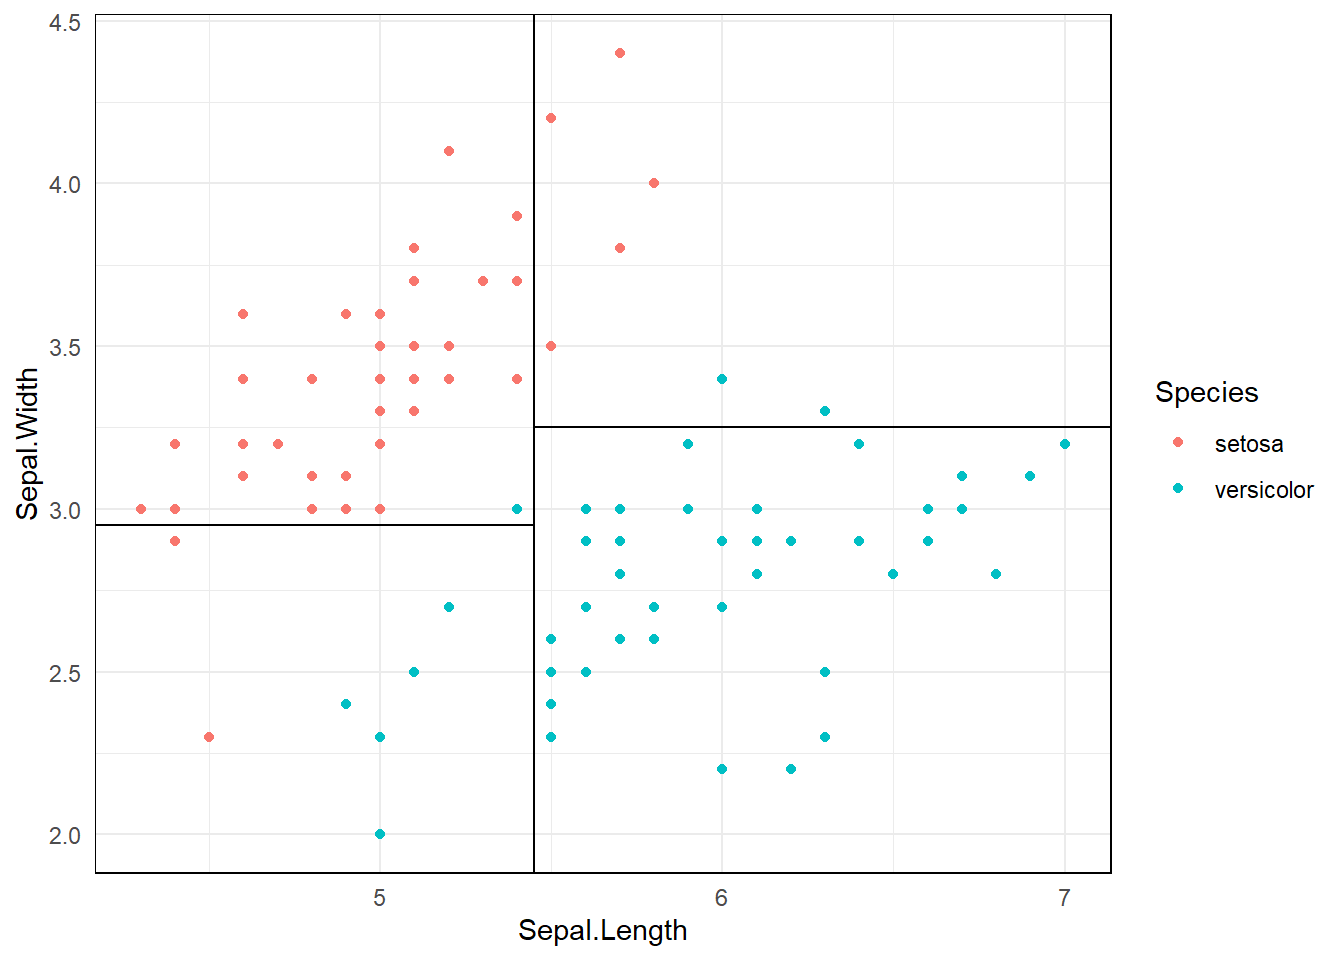
\includegraphics[keepaspectratio]{ch3_files/figure-pdf/unnamed-chunk-5-2.pdf}}

\pandocbounded{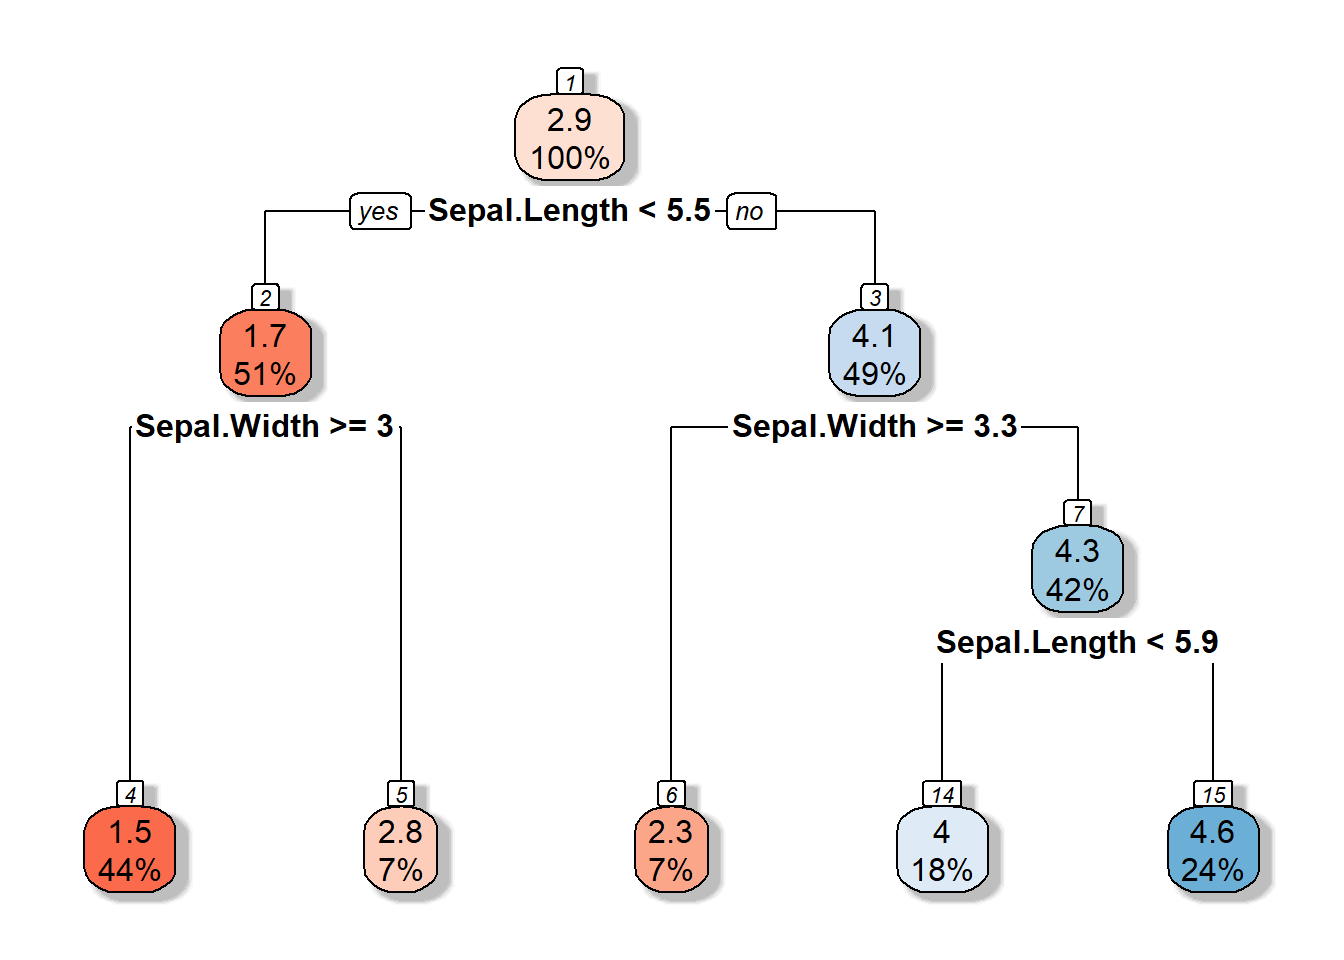
\includegraphics[keepaspectratio]{ch3_files/figure-pdf/unnamed-chunk-6-1.pdf}}

\pandocbounded{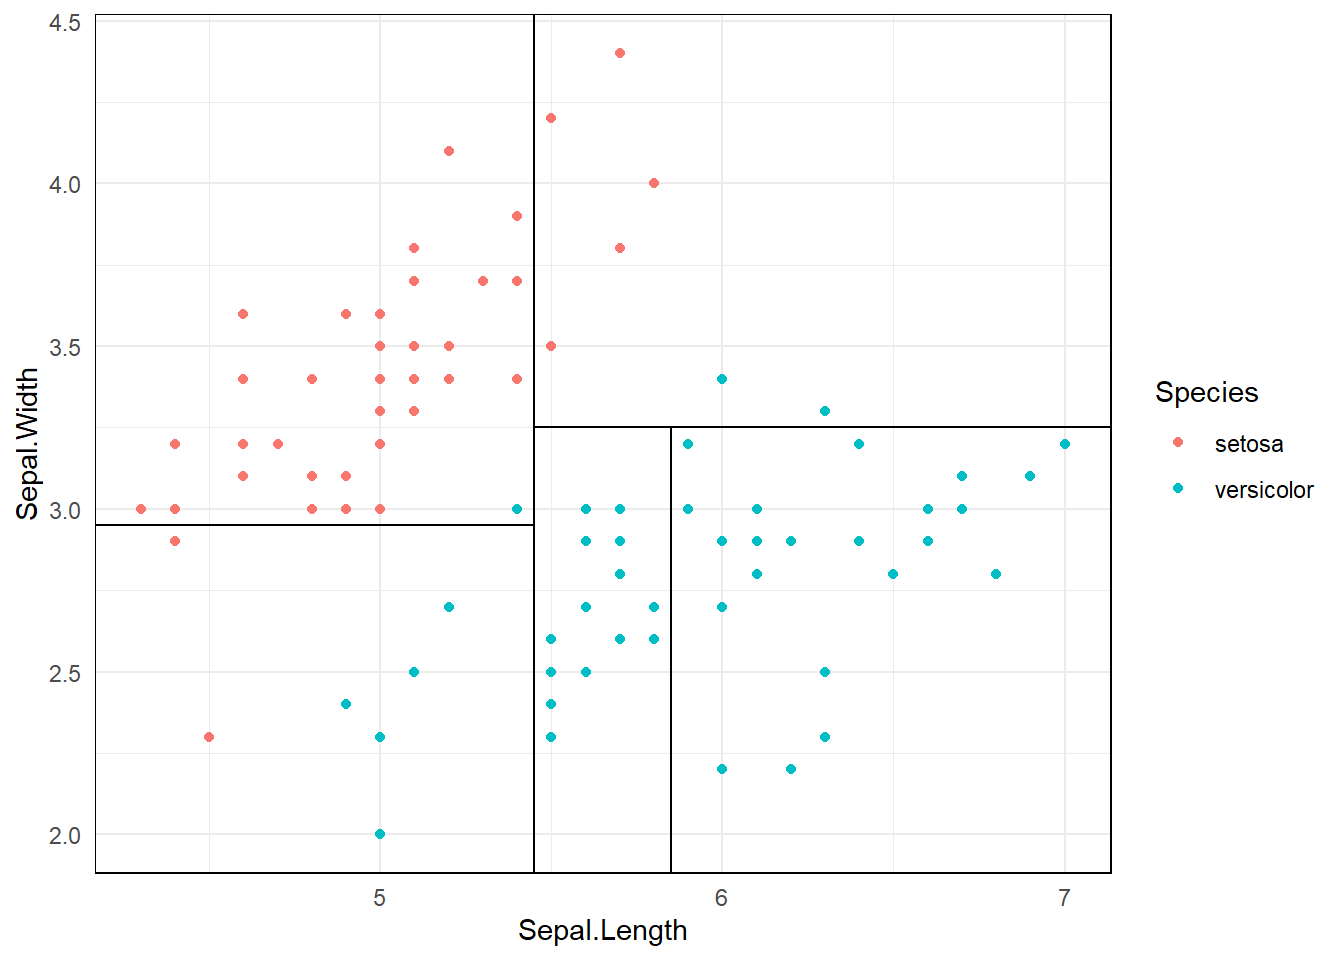
\includegraphics[keepaspectratio]{ch3_files/figure-pdf/unnamed-chunk-6-2.pdf}}

\section{Pruning Regression Trees}\label{pruning-regression-trees}

Once a regression tree is grown, it often becomes \textbf{too complex}
--- it may fit the training data very well but perform poorly on new,
unseen data.\\
This problem is known as \textbf{overfitting}.

\textbf{Pruning} is the process of \textbf{reducing the size} of a fully
grown tree to improve its ability to generalize.

\subsection{Why Prune?}\label{why-prune}

\begin{itemize}
\tightlist
\item
  A large tree captures \textbf{noise} as if it were structure.\\
\item
  It has \textbf{low bias} but \textbf{high variance}.\\
\item
  Pruning helps to find a \textbf{balance between model complexity and
  prediction accuracy}.
\end{itemize}

\subsection{Types of Pruning}\label{types-of-pruning}

There are two main approaches:

\subsubsection{(a) Pre-pruning (Early
stopping)}\label{a-pre-pruning-early-stopping}

Stop the tree growth \textbf{before} it becomes too large.

Common stopping rules:

\begin{itemize}
\item
  Minimum number of observations in a node
\item
  Maximum tree depth
\item
  Minimum decrease in SSE required for a split
\end{itemize}

\subsubsection{(b) Post-pruning (Cost Complexity
Pruning)}\label{b-post-pruning-cost-complexity-pruning}

Grow a \textbf{large tree first}, then prune it \textbf{backward} by
removing branches that contribute little to predictive accuracy.

\subsection{Cost Complexity Pruning (a.k.a. Weakest Link
Pruning)}\label{cost-complexity-pruning-a.k.a.-weakest-link-pruning}

The idea is to penalize tree size using a complexity parameter
(\(\lambda\)).

For any subtree ( T ):

\[
C(T) = \text{Error}(T) + \lambda L(T)
\]

where:

\begin{itemize}
\tightlist
\item
  \text{Error}(T): measure of fit (e.g., sum of squared errors)\\
\item
  \(L(T)\): number of leaf nodes in the tree (measure of complexity)\\
\item
  \(\lambda\): penalty factor controlling the trade-off between
  complexity and predictive power
\end{itemize}

\subsection{Interpretation of
Parameters}\label{interpretation-of-parameters}

\begin{longtable}[]{@{}
  >{\raggedright\arraybackslash}p{(\linewidth - 2\tabcolsep) * \real{0.5455}}
  >{\raggedright\arraybackslash}p{(\linewidth - 2\tabcolsep) * \real{0.4545}}@{}}
\toprule\noalign{}
\begin{minipage}[b]{\linewidth}\raggedright
Parameter
\end{minipage} & \begin{minipage}[b]{\linewidth}\raggedright
Meaning
\end{minipage} \\
\midrule\noalign{}
\endhead
\bottomrule\noalign{}
\endlastfoot
\(\lambda = 0\) & Fully grown decision tree (no penalty for
complexity). \\
\(\lambda = \infty\) & Root node only (maximum penalty, no splits). \\
\(0 < \lambda < \infty\) & Balances predictive power and complexity. \\
\end{longtable}

\subsection{Total Cost Components}\label{total-cost-components}

\[
\text{Total Cost} = \text{Measure of Fit} + \text{Measure of Complexity}
\]

\begin{itemize}
\tightlist
\item
  \textbf{Measure of Fit:} Error (e.g., SSE)\\
\item
  \textbf{Measure of Complexity:} Number of leaf nodes \(L(T)\)
\end{itemize}

So, \[
C(T) = \text{Error}(T) + \lambda L(T)
\]

This is sometimes written as:

\[
R_\lambda(T) = R(T) + \lambda |T|
\]

Both expressions represent the same concept --- a \textbf{trade-off
between model fit and simplicity}.

\section{Example R code for Pre-pruning and
Post-pruning}\label{example-r-code-for-pre-pruning-and-post-pruning}

\begin{Shaded}
\begin{Highlighting}[]
\CommentTok{\# Load necessary packages}
\FunctionTok{library}\NormalTok{(rpart)}
\FunctionTok{library}\NormalTok{(rpart.plot)}

\CommentTok{\# Use built{-}in dataset}
\FunctionTok{data}\NormalTok{(mtcars)}

\CommentTok{\# {-}{-}{-}{-}{-}{-}{-}{-}{-}{-}{-}{-}{-}{-}{-}{-}{-}{-}{-}{-}{-}{-}{-}{-}{-}{-}{-}{-}{-}}
\CommentTok{\# 🌱 1. Pre{-}pruning (Early stopping)}
\CommentTok{\# {-}{-}{-}{-}{-}{-}{-}{-}{-}{-}{-}{-}{-}{-}{-}{-}{-}{-}{-}{-}{-}{-}{-}{-}{-}{-}{-}{-}{-}}
\CommentTok{\# Control parameters limit tree growth}
\NormalTok{prepruned\_tree }\OtherTok{\textless{}{-}} \FunctionTok{rpart}\NormalTok{(}
\NormalTok{  mpg }\SpecialCharTok{\textasciitilde{}}\NormalTok{ ., }
  \AttributeTok{data =}\NormalTok{ mtcars,}
  \AttributeTok{method =} \StringTok{"anova"}\NormalTok{,}
  \AttributeTok{control =} \FunctionTok{rpart.control}\NormalTok{(}
    \AttributeTok{minsplit =} \DecValTok{10}\NormalTok{,   }\CommentTok{\# minimum observations required to attempt a split}
    \AttributeTok{cp =} \FloatTok{0.02}\NormalTok{,       }\CommentTok{\# minimum improvement in SSE required for a split}
    \AttributeTok{maxdepth =} \DecValTok{3}     \CommentTok{\# maximum depth of the tree}
\NormalTok{  )}
\NormalTok{)}

\CommentTok{\# Visualize the pre{-}pruned tree}
\FunctionTok{rpart.plot}\NormalTok{(prepruned\_tree, }\AttributeTok{main =} \StringTok{"Pre{-}pruned Regression Tree"}\NormalTok{)}
\end{Highlighting}
\end{Shaded}

\pandocbounded{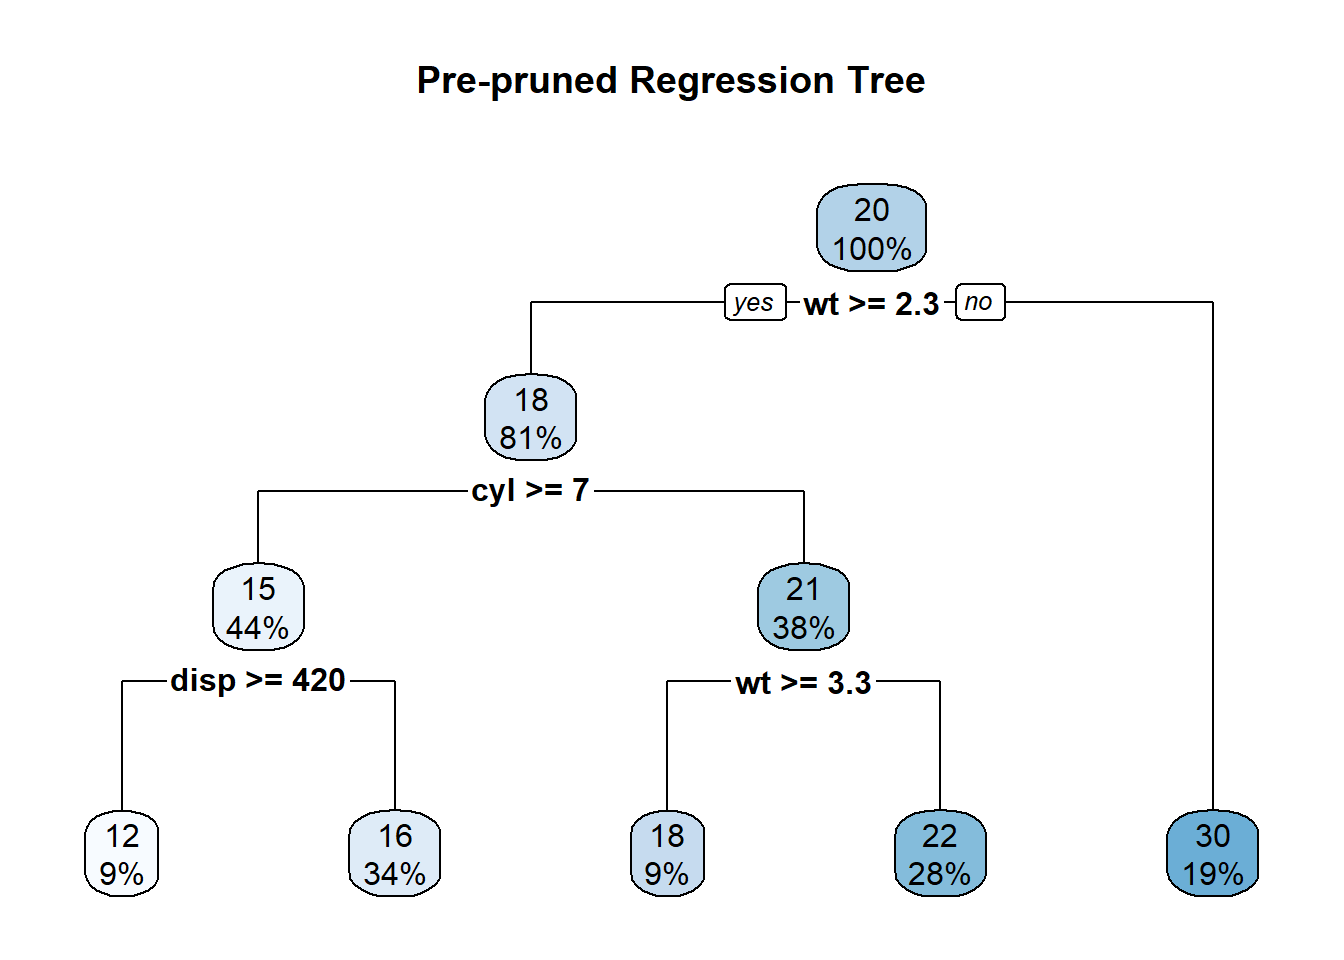
\includegraphics[keepaspectratio]{ch3_files/figure-pdf/unnamed-chunk-7-1.pdf}}

\begin{Shaded}
\begin{Highlighting}[]
\CommentTok{\# Print summary}
\FunctionTok{print}\NormalTok{(prepruned\_tree)}
\end{Highlighting}
\end{Shaded}

\begin{verbatim}
n= 32 

node), split, n, deviance, yval
      * denotes terminal node

 1) root 32 1126.047000 20.09062  
   2) wt>=2.26 26  346.566500 17.78846  
     4) cyl>=7 14   85.200000 15.10000  
       8) disp>=420 3   12.326670 11.83333 *
       9) disp< 420 11   32.129090 15.99091 *
     5) cyl< 7 12   42.122500 20.92500  
      10) wt>=3.3275 3    1.086667 18.36667 *
      11) wt< 3.3275 9   14.855560 21.77778 *
   3) wt< 2.26 6   44.553330 30.06667 *
\end{verbatim}

\begin{Shaded}
\begin{Highlighting}[]
\FunctionTok{summary}\NormalTok{(prepruned\_tree)}
\end{Highlighting}
\end{Shaded}

\begin{verbatim}
Call:
rpart(formula = mpg ~ ., data = mtcars, method = "anova", control = rpart.control(minsplit = 10, 
    cp = 0.02, maxdepth = 3))
  n= 32 

          CP nsplit rel error    xerror       xstd
1 0.65266121      0 1.0000000 1.1014883 0.25751457
2 0.19470235      1 0.3473388 0.5716426 0.15470821
3 0.03618342      2 0.1526364 0.3772224 0.09990268
4 0.02324972      3 0.1164530 0.3314091 0.09620281
5 0.02000000      4 0.0932033 0.3104538 0.09455554

Variable importance
  wt disp   hp drat  cyl qsec   vs 
  27   25   19   11    9    5    5 

Node number 1: 32 observations,    complexity param=0.6526612
  mean=20.09062, MSE=35.18897 
  left son=2 (26 obs) right son=3 (6 obs)
  Primary splits:
      wt   < 2.26   to the right, improve=0.6526612, (0 missing)
      cyl  < 5      to the right, improve=0.6431252, (0 missing)
      disp < 163.8  to the right, improve=0.6130502, (0 missing)
      hp   < 118    to the right, improve=0.6010712, (0 missing)
      vs   < 0.5    to the left,  improve=0.4409477, (0 missing)
  Surrogate splits:
      disp < 101.55 to the right, agree=0.969, adj=0.833, (0 split)
      hp   < 92     to the right, agree=0.938, adj=0.667, (0 split)
      drat < 4      to the left,  agree=0.906, adj=0.500, (0 split)
      cyl  < 5      to the right, agree=0.844, adj=0.167, (0 split)

Node number 2: 26 observations,    complexity param=0.1947024
  mean=17.78846, MSE=13.32948 
  left son=4 (14 obs) right son=5 (12 obs)
  Primary splits:
      cyl  < 7      to the right, improve=0.6326174, (0 missing)
      disp < 266.9  to the right, improve=0.6326174, (0 missing)
      hp   < 136.5  to the right, improve=0.5803554, (0 missing)
      wt   < 3.325  to the right, improve=0.5393370, (0 missing)
      qsec < 18.15  to the left,  improve=0.4210605, (0 missing)
  Surrogate splits:
      disp < 266.9  to the right, agree=1.000, adj=1.000, (0 split)
      hp   < 136.5  to the right, agree=0.962, adj=0.917, (0 split)
      wt   < 3.49   to the right, agree=0.885, adj=0.750, (0 split)
      qsec < 18.15  to the left,  agree=0.885, adj=0.750, (0 split)
      vs   < 0.5    to the left,  agree=0.885, adj=0.750, (0 split)

Node number 3: 6 observations
  mean=30.06667, MSE=7.425556 

Node number 4: 14 observations,    complexity param=0.03618342
  mean=15.1, MSE=6.085714 
  left son=8 (3 obs) right son=9 (11 obs)
  Primary splits:
      disp < 420    to the right, improve=0.4782188, (0 missing)
      wt   < 4.66   to the right, improve=0.4782188, (0 missing)
      hp   < 192.5  to the right, improve=0.4669349, (0 missing)
      carb < 3.5    to the right, improve=0.4669349, (0 missing)
      qsec < 17.71  to the right, improve=0.4306658, (0 missing)
  Surrogate splits:
      wt   < 4.66   to the right, agree=1.000, adj=1.000, (0 split)
      drat < 3.035  to the left,  agree=0.857, adj=0.333, (0 split)
      qsec < 17.41  to the right, agree=0.857, adj=0.333, (0 split)

Node number 5: 12 observations,    complexity param=0.02324972
  mean=20.925, MSE=3.510208 
  left son=10 (3 obs) right son=11 (9 obs)
  Primary splits:
      wt   < 3.3275 to the right, improve=0.6215272, (0 missing)
      cyl  < 5      to the right, improve=0.5573591, (0 missing)
      hp   < 96     to the right, improve=0.5507811, (0 missing)
      disp < 163.8  to the right, improve=0.4615111, (0 missing)
      carb < 3      to the right, improve=0.2857431, (0 missing)
  Surrogate splits:
      disp < 163.8  to the right, agree=0.917, adj=0.667, (0 split)
      hp   < 116.5  to the right, agree=0.833, adj=0.333, (0 split)

Node number 8: 3 observations
  mean=11.83333, MSE=4.108889 

Node number 9: 11 observations
  mean=15.99091, MSE=2.920826 

Node number 10: 3 observations
  mean=18.36667, MSE=0.3622222 

Node number 11: 9 observations
  mean=21.77778, MSE=1.650617 
\end{verbatim}

\begin{Shaded}
\begin{Highlighting}[]
\CommentTok{\# {-}{-}{-}{-}{-}{-}{-}{-}{-}{-}{-}{-}{-}{-}{-}{-}{-}{-}{-}{-}{-}{-}{-}{-}{-}{-}{-}{-}{-}}
\CommentTok{\# 🌳 2. Post{-}pruning (Cost{-}complexity pruning)}
\CommentTok{\# {-}{-}{-}{-}{-}{-}{-}{-}{-}{-}{-}{-}{-}{-}{-}{-}{-}{-}{-}{-}{-}{-}{-}{-}{-}{-}{-}{-}{-}}
\CommentTok{\# Step 1: Grow a large tree first}
\NormalTok{full\_tree }\OtherTok{\textless{}{-}} \FunctionTok{rpart}\NormalTok{(}
\NormalTok{  mpg }\SpecialCharTok{\textasciitilde{}}\NormalTok{ ., }
  \AttributeTok{data =}\NormalTok{ mtcars,}
  \AttributeTok{method =} \StringTok{"anova"}\NormalTok{,}
  \AttributeTok{control =} \FunctionTok{rpart.control}\NormalTok{(}\AttributeTok{cp =} \FloatTok{0.0001}\NormalTok{)  }\CommentTok{\# allow the tree to grow large}
\NormalTok{)}

\CommentTok{\# Step 2: Display complexity parameter (CP) table}
\FunctionTok{printcp}\NormalTok{(full\_tree)}
\end{Highlighting}
\end{Shaded}

\begin{verbatim}

Regression tree:
rpart(formula = mpg ~ ., data = mtcars, method = "anova", control = rpart.control(cp = 1e-04))

Variables actually used in tree construction:
[1] cyl hp 

Root node error: 1126/32 = 35.189

n= 32 

        CP nsplit rel error  xerror    xstd
1 0.643125      0   1.00000 1.05398 0.25284
2 0.097484      1   0.35687 0.66363 0.16803
3 0.000100      2   0.25939 0.58164 0.11140
\end{verbatim}

\begin{Shaded}
\begin{Highlighting}[]
\CommentTok{\# Step 3: Plot cross{-}validation results}
\FunctionTok{plotcp}\NormalTok{(full\_tree, }\AttributeTok{main =} \StringTok{"Cost{-}Complexity Pruning Plot"}\NormalTok{)}
\end{Highlighting}
\end{Shaded}

\pandocbounded{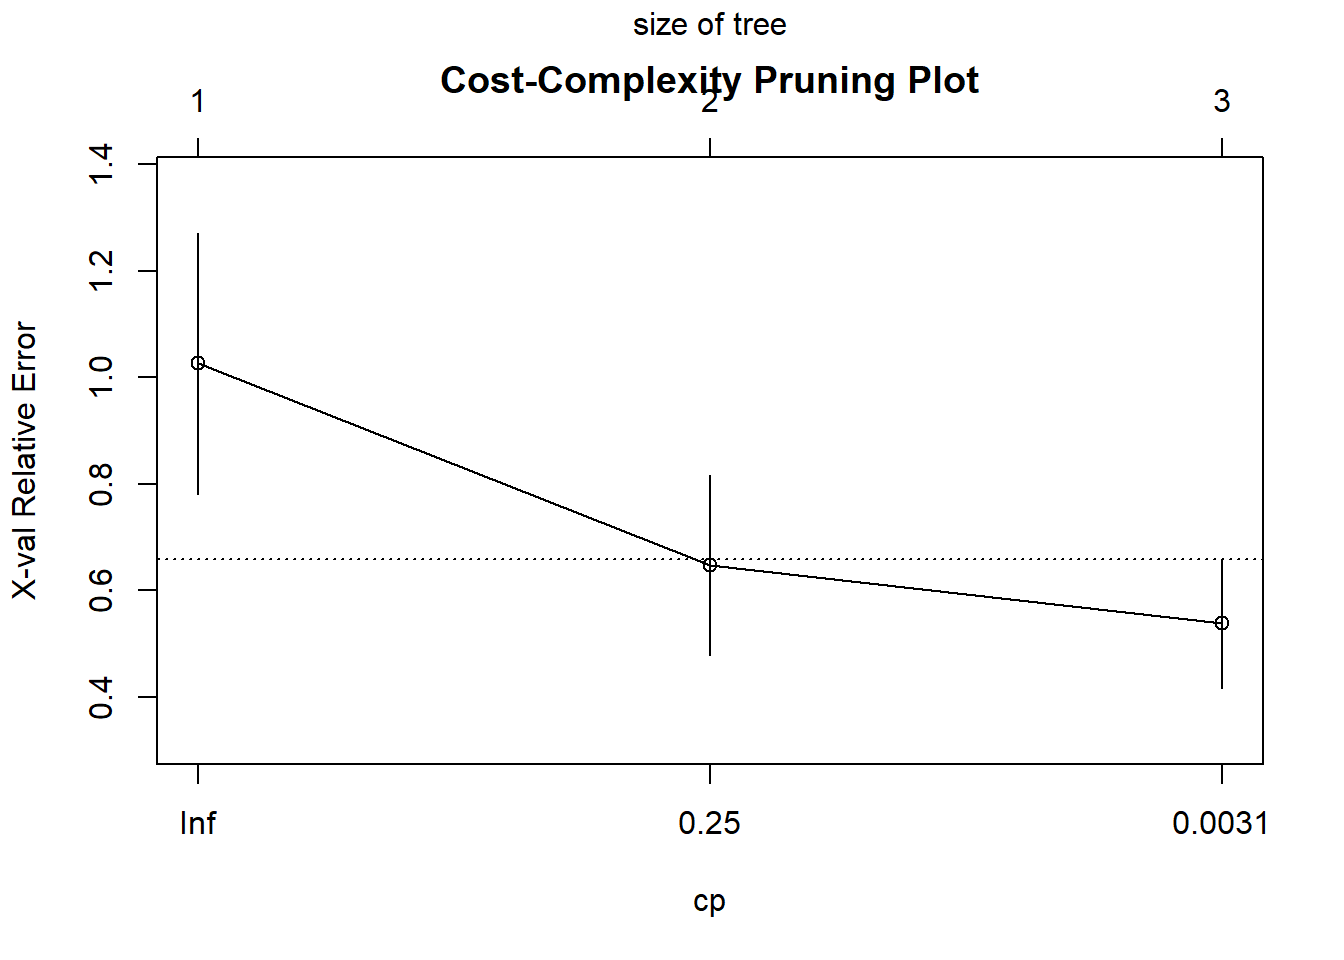
\includegraphics[keepaspectratio]{ch3_files/figure-pdf/unnamed-chunk-7-2.pdf}}

\begin{Shaded}
\begin{Highlighting}[]
\CommentTok{\# Step 4: Select the cp value that minimizes cross{-}validation error}
\NormalTok{optimal\_cp }\OtherTok{\textless{}{-}}\NormalTok{ full\_tree}\SpecialCharTok{$}\NormalTok{cptable[}\FunctionTok{which.min}\NormalTok{(full\_tree}\SpecialCharTok{$}\NormalTok{cptable[,}\StringTok{"xerror"}\NormalTok{]), }\StringTok{"CP"}\NormalTok{]}

\CommentTok{\# Step 5: Prune the tree at the optimal cp value}
\NormalTok{pruned\_tree }\OtherTok{\textless{}{-}} \FunctionTok{prune}\NormalTok{(full\_tree, }\AttributeTok{cp =}\NormalTok{ optimal\_cp)}

\CommentTok{\# Step 6: Visualize the pruned tree}
\FunctionTok{rpart.plot}\NormalTok{(pruned\_tree, }\AttributeTok{main =} \StringTok{"Post{-}pruned Regression Tree"}\NormalTok{)}
\end{Highlighting}
\end{Shaded}

\pandocbounded{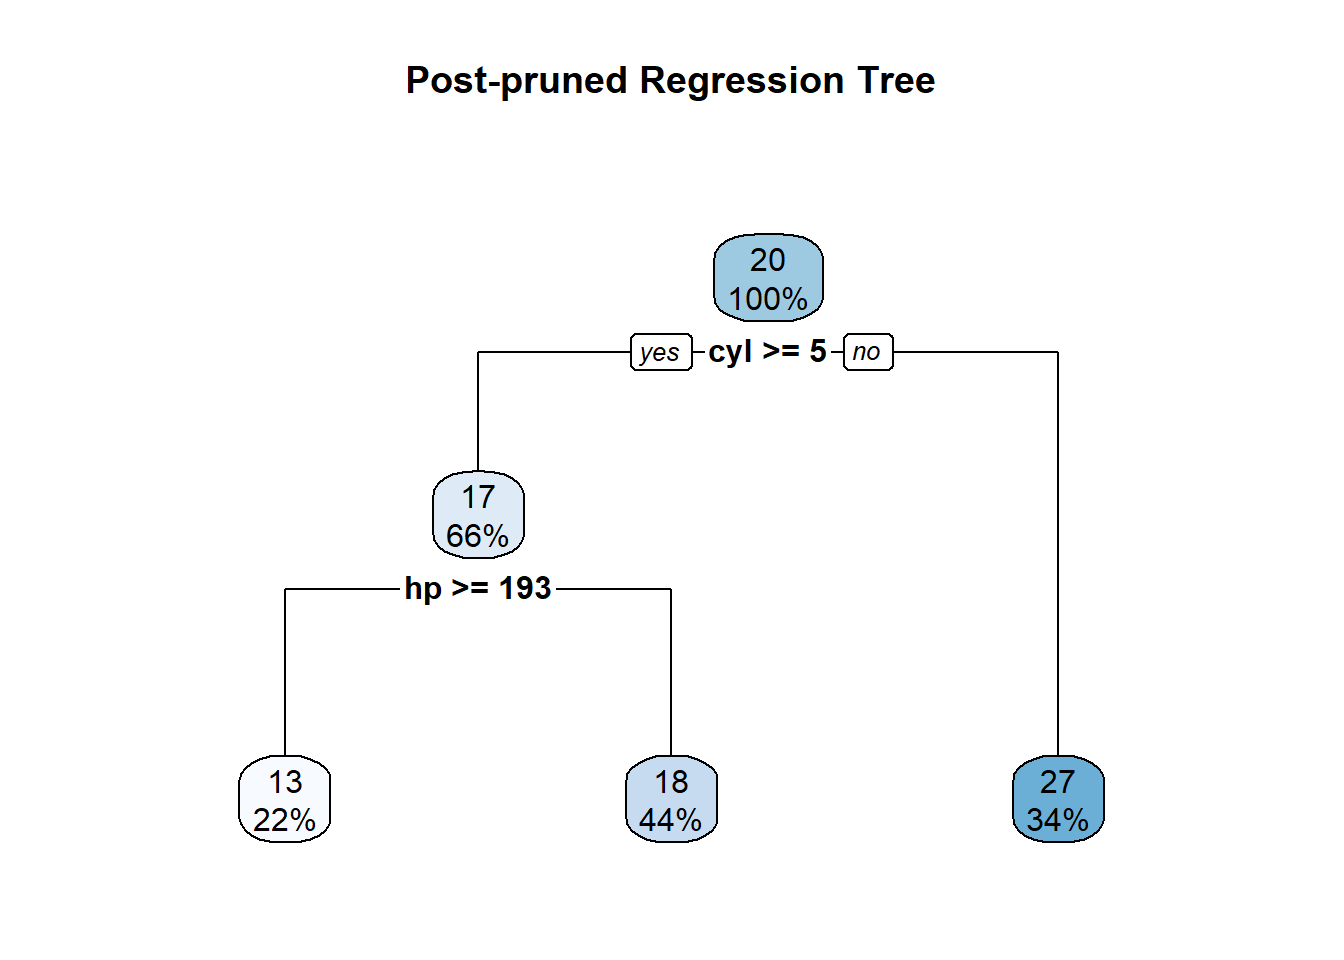
\includegraphics[keepaspectratio]{ch3_files/figure-pdf/unnamed-chunk-7-3.pdf}}

\begin{Shaded}
\begin{Highlighting}[]
\CommentTok{\# Step 7: Summarize pruned model}
\FunctionTok{summary}\NormalTok{(pruned\_tree)}
\end{Highlighting}
\end{Shaded}

\begin{verbatim}
Call:
rpart(formula = mpg ~ ., data = mtcars, method = "anova", control = rpart.control(cp = 1e-04))
  n= 32 

          CP nsplit rel error    xerror      xstd
1 0.64312523      0 1.0000000 1.0539777 0.2528389
2 0.09748407      1 0.3568748 0.6636336 0.1680308
3 0.00010000      2 0.2593907 0.5816401 0.1113953

Variable importance
 cyl disp   hp   wt qsec   vs carb 
  20   20   19   16   12   11    1 

Node number 1: 32 observations,    complexity param=0.6431252
  mean=20.09062, MSE=35.18897 
  left son=2 (21 obs) right son=3 (11 obs)
  Primary splits:
      cyl  < 5      to the right, improve=0.6431252, (0 missing)
      wt   < 2.3925 to the right, improve=0.6356630, (0 missing)
      disp < 163.8  to the right, improve=0.6130502, (0 missing)
      hp   < 118    to the right, improve=0.6010712, (0 missing)
      vs   < 0.5    to the left,  improve=0.4409477, (0 missing)
  Surrogate splits:
      disp < 142.9  to the right, agree=0.969, adj=0.909, (0 split)
      hp   < 101    to the right, agree=0.938, adj=0.818, (0 split)
      wt   < 2.5425 to the right, agree=0.906, adj=0.727, (0 split)
      qsec < 18.41  to the left,  agree=0.844, adj=0.545, (0 split)
      vs   < 0.5    to the left,  agree=0.844, adj=0.545, (0 split)

Node number 2: 21 observations,    complexity param=0.09748407
  mean=16.64762, MSE=9.451066 
  left son=4 (7 obs) right son=5 (14 obs)
  Primary splits:
      hp   < 192.5  to the right, improve=0.5530828, (0 missing)
      cyl  < 7      to the right, improve=0.5068475, (0 missing)
      disp < 266.9  to the right, improve=0.5068475, (0 missing)
      wt   < 3.49   to the right, improve=0.4414890, (0 missing)
      drat < 3.075  to the left,  improve=0.1890739, (0 missing)
  Surrogate splits:
      disp < 334    to the right, agree=0.857, adj=0.571, (0 split)
      wt   < 4.66   to the right, agree=0.810, adj=0.429, (0 split)
      qsec < 15.455 to the left,  agree=0.810, adj=0.429, (0 split)
      carb < 3.5    to the right, agree=0.762, adj=0.286, (0 split)
      gear < 4.5    to the right, agree=0.714, adj=0.143, (0 split)

Node number 3: 11 observations
  mean=26.66364, MSE=18.48959 

Node number 4: 7 observations
  mean=13.41429, MSE=4.118367 

Node number 5: 14 observations
  mean=18.26429, MSE=4.276582 
\end{verbatim}

\section{Classification Trees: Best Split, Entropy, and Gini
Coefficients}\label{classification-trees-best-split-entropy-and-gini-coefficients}

Classification trees are used when the response variable is
\textbf{categorical}.\\
At each node, the algorithm tries to find the \textbf{best split} ---
the one that produces the most \textbf{homogeneous} (pure) child nodes.

\subsection{The Idea of ``Best Split''}\label{the-idea-of-best-split}

At any node in the tree:

\begin{itemize}
\tightlist
\item
  The data are divided into two (or more) groups based on a predictor.
\item
  The \textbf{best split} is the one that makes each resulting group as
  \textbf{pure} as possible with respect to the class labels.
\end{itemize}

To measure \textbf{purity}, we use \textbf{impurity measures} such as:

\begin{itemize}
\item
  \textbf{Entropy}
\item
  \textbf{Gini index}
\item
  (Sometimes) \textbf{Misclassification error}
\end{itemize}

\subsection{Entropy}\label{entropy}

Entropy measures the \textbf{disorder} or \textbf{uncertainty} in a
node.

If there are ( K ) classes and ( p\_k ) is the proportion of
observations belonging to class ( k ), then:

\[
\text{Entropy} = - \sum_{k=1}^{K} p_k \log_2(p_k)
\]

\subsubsection{Properties:}\label{properties}

\begin{itemize}
\tightlist
\item
  Entropy = 0 → Node is perfectly pure (all observations belong to one
  class).
\item
  Entropy is maximum when all classes are equally likely.
\end{itemize}

\subsubsection{Example:}\label{example}

\begin{longtable}[]{@{}llll@{}}
\toprule\noalign{}
Class & Count & \(p_k\) & \(-p_k \log_2(p_k)\) \\
\midrule\noalign{}
\endhead
\bottomrule\noalign{}
\endlastfoot
A & 8 & 0.8 & 0.257 \\
B & 2 & 0.2 & 0.464 \\
\end{longtable}

\[
\text{Entropy} = 0.257 + 0.464 = 0.721
\]

\subsection{Gini Index}\label{gini-index}

The \textbf{Gini coefficient} (or \textbf{Gini impurity}) is another
measure of node impurity.

\[
\text{Gini} = 1 - \sum_{k=1}^{K} p_k^2
\]

\subsubsection{Properties:}\label{properties-1}

\begin{itemize}
\item
  Gini = 0 → Perfectly pure node
\item
  Gini is smaller when the node is more homogeneous
\end{itemize}

\subsubsection{Example:}\label{example-1}

Using the same proportions as above ( \(p_1 = 0.8, p_2 = 0.2\) ):

\[
\text{Gini} = 1 - (0.8^2 + 0.2^2) = 1 - (0.64 + 0.04) = 0.32
\]

\subsection{Misclassification Error (less
common)}\label{misclassification-error-less-common}

A simpler impurity measure sometimes used:

\[
\text{Error} = 1 - \max(p_k)
\]

For the same node ( \(\max(p_k) = 0.8\) ):

\[
\text{Error} = 1 - 0.8 = 0.2
\]

\subsection{Choosing the Best Split}\label{choosing-the-best-split}

For each possible split:

\begin{enumerate}
\def\labelenumi{\arabic{enumi}.}
\item
  Compute the impurity (Entropy or Gini) \textbf{before} splitting ---
  call this \(I_{\text{parent}}\).
\item
  Compute the impurity of the \textbf{child nodes} (weighted by their
  sizes):
\end{enumerate}

\[
I_{\text{split}} = \frac{n_L}{n} I_L + \frac{n_R}{n} I_R
\]

\begin{enumerate}
\def\labelenumi{\arabic{enumi}.}
\setcounter{enumi}{2}
\tightlist
\item
  Compute the \textbf{information gain} (reduction in impurity):
\end{enumerate}

\[
\text{Gain} = I_{\text{parent}} - I_{\text{split}}
\]

\begin{enumerate}
\def\labelenumi{\arabic{enumi}.}
\setcounter{enumi}{3}
\tightlist
\item
  The \textbf{best split} is the one that maximizes this gain (i.e.,
  gives the largest reduction in impurity).
\end{enumerate}

\subsection{Comparing Entropy and
Gini}\label{comparing-entropy-and-gini}

\begin{longtable}[]{@{}
  >{\raggedright\arraybackslash}p{(\linewidth - 4\tabcolsep) * \real{0.4074}}
  >{\raggedright\arraybackslash}p{(\linewidth - 4\tabcolsep) * \real{0.3704}}
  >{\raggedright\arraybackslash}p{(\linewidth - 4\tabcolsep) * \real{0.2222}}@{}}
\toprule\noalign{}
\begin{minipage}[b]{\linewidth}\raggedright
Property
\end{minipage} & \begin{minipage}[b]{\linewidth}\raggedright
Entropy
\end{minipage} & \begin{minipage}[b]{\linewidth}\raggedright
Gini
\end{minipage} \\
\midrule\noalign{}
\endhead
\bottomrule\noalign{}
\endlastfoot
Range & 0 to 1 & 0 to 0.5 \\
Shape & Logarithmic & Quadratic \\
Interpretation & Information theory measure & Probability of
misclassification \\
Behavior & Slightly more sensitive to rare classes & Computationally
simpler \\
Commonly used in & C4.5, ID3 algorithms & CART algorithm \\
\end{longtable}

Both criteria often lead to \textbf{similar splits} in practice.

\bookmarksetup{startatroot}

\chapter*{References}\label{references}
\addcontentsline{toc}{chapter}{References}

\markboth{References}{References}

\phantomsection\label{refs}
\begin{CSLReferences}{0}{1}
\end{CSLReferences}




\end{document}
